\section{Primo approccio: modello lineare}

\subsection{Workspace}

Prima di iniziare a parlare del modello adottato per prevedere la richiesta di
\emph{Bike sharing}, è opportuno chiarire come verranno gestite le variabili
coinvolte durante l'analisi dei dati.

\subsubsection{Variabili esplicative}\label{sec:modlin-work-espl}
Per quanto riguarda le variabili esplicative, \texttt{holiday},
\texttt{working day}, \texttt{weather}, \texttt{temp}, \texttt{atemp},
\texttt{humidity}, \texttt{windspeed} non verranno trasformate in alcun modo.
In particolare:

\begin{itemize}
\item \texttt{holiday}, pur essendo qualitativa, è già espressa in un formato
  accettabile, ovvero \textbf{0} per una modalità (\textbf{N}) e \textbf{1}
  per l'altra (\textbf{S});
\item il caso di \texttt{workingday} è totalmente analogo a quello di
  \texttt{holiday};
\item \texttt{weather}, pur prevedendo quattro modalità, si può vedere come
  una variabile quantitativa per la quale più alto è il valore, peggiore è il
  tempo (con valori compresi tra quelli nominati nella sezione
  \ref{sec:intro-dati}).
\end{itemize}

\paragraph{Variabili trasformate} \mbox{}\\
Non tutte le variabili in gioco erano fornite in modo tale da essere
analizzate con semplicità.
Le restanti variabili esplicative sono state modificate con i seguenti criteri:

\begin{itemize}
\item \texttt{datetime} conteneva al suo interno il giorno e l'ora.
  Dopo una rapida analisi del dataset, si è notato che tutte le ore erano in
  realtà nel formato ``HH:00:00'', deducendo che si trattasse di misurazioni
  orarie. \\
  Oltre a ciò è stato considerato che la richiesta del servizio di \emph{Bike
  sharing} non dipende strettamente da un giorno particolare (e.g. 2012-07-04),
  ma principalmente dalla stagione a cui questo apparteneva e al fatto che
  questo fosse festivo e/o feriale o meno, fattori già presenti in altre
  variabili esplicative. \\
  A maggior ragione, lo scopo finale del modello era quello di effettuare
  previsioni su giorni non presenti nel dataset, perciò riuscire a costruire
  un modello che restituisse previsioni corrette su un giorno di cui si
  conoscevano già i risultati non era significativo, mentre il trend con cui
  il servizio viene richiesto durante una giornata potrebbe esserlo. \\
  Di conseguenza, si è ritenuto opportuno trasformare \texttt{datetime} in una
  variabile con valori interi uguali ad HH (ignorando completamente il
  giorno), con valori perciò compresi tra 0 (mezzanotte) e 23 (11:00 PM);
\item \texttt{season} presentava quattro possibili modalità. A differenza di
  \texttt{weather}, le cui modalità potevano essere viste come un insieme
  ordinato, non si vede alcun ordine per le stagioni. \\
  Un possibile tentativo sarebbe stato, in modo del tutto analogo a
  \texttt{weather}, pensare a un insieme dove al valore minimo sarebbe
  corrisposta la stagione caratterizzata da temperature più fredde e da
  condizioni metereologiche peggiori e viceversa per il valore massimo. \\
  Tuttavia, questo approccio non è stato considerato valido poichè primavera e
  autunno sono simili da questo punto di vista. \\
  Si è proceduto creando due nuove variabili, \texttt{season.summer} e
  \texttt{season.fall}, così che la variabile originaria \texttt{summer} fosse
  riorganizzata nel seguente modo:
  \begin{itemize}
  \item \texttt{season} variabile che vale 1 se la stagione è primavera
    (modalità \textbf{1} per la variabile originaria)
  \item \texttt{season.summer} variabile che vale 1 se la stagione è primavera
    (modalità \textbf{2} per la variabile originaria)
  \item \texttt{season.fall} variabile che vale 1 se la stagione è primavera
    (modalità \textbf{3} per la variabile originaria)
  \item  \texttt{season}, \texttt{season.summer} e \texttt{season.fall} con
    valore 0 se la stagione è inverno (modalità \textbf{4} per la variabile
    originaria)
  \end{itemize}
\end{itemize}

Tali trasformazioni sono state applicate durante il popolamento del dataset, il
cui script è stato riportato in sezione \ref{sec:script-populate}.

In fondo allo script si possono notare alcune costanti che vengono settate per
il workspace: si tratta di \texttt{columns}, ovvero i nomi delle variabili
esplicative utilizzate, e di altre costanti il cui uso verrà spiegato più
dettagliatamente in seguito.

\subsubsection{Variabili risposta}
Per le variabili risposta, è stato scelto di considerare solo
\texttt{train\$count}, poichè lo studio dei modelli per le variabili
\texttt{train\$registered} e \texttt{train\$casual} è del tutto analogo a
quello della variabile che insieme compongono.

\subsection{Modello lineare}\label{sec:mod-lin}
Dopo aver impostato correttamente il workspace, si può procedere calcolando il
modello lineare semplice $ y = \beta{}_0 + \beta{}_1 \cdot{} x + \epsilon{} $
per tutte le variabili, dove y è train\$count e x una delle variabili
esplicative.
Inizialmente questa operazione viene ripetuta con il comando \texttt{train.lm
= lm(y $ \sim{} $ x)} per tutte le variabili esplicative, ottenendo il
risultato migliore per x = train\$datetime.

Questo risultato ci può dare garanzie sulla buona intuizione riguardo il
formato scelto per la variabile \texttt{datetime}, spiegato nella sezione
\ref{sec:modlin-work-espl}, ovvero che l'ora è uno dei fattori che incidono
molto sulla richiesta del servizio di \emph{Bike sharing}.

Tale considerazione può essere compresa guardando i valori dei residui visibili
grazie alla visione d'insieme del modello lineare fornita dal comando
\texttt{summary()}.

\begin{figure}[H]\label{fig:simplest-linear-model}
  \centering
  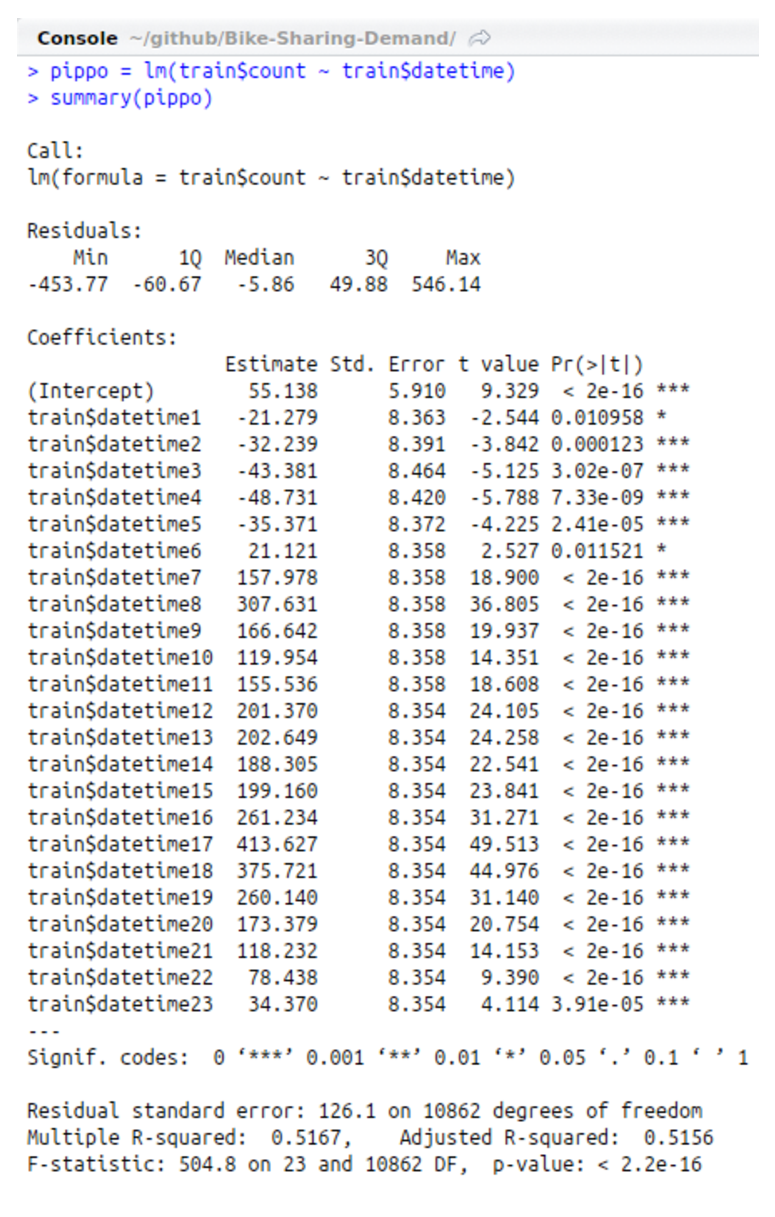
\includegraphics[width=.7\columnwidth]{images/simplest-linear-model.eps}
  \caption{Modello lineare con \texttt{train\$datetime}}
\end{figure}

I dati relativi al modello lineare appena individuato potrebbero ingenuamente
suggerire che la stima individuata per il coefficiente $\beta{}_1$ sia buona,
visto un valore molto elevato della statistica F e, di conseguenza, un p-value
prossimo a 0.

Tuttavia, richiedendo i grafici relativi al modello lineare, è ben facile
intuire che il modello lineare calcolato non è affatto soddisfacente, poichè è
evidente che gli errori non seguono distribuzione normale secondo
questo modello:

\begin{itemize}
\item I residui, sebbene abbiano media nulla, non sembrano omoschedastici;
  oltre a questo, pare anche che il modello non riesca a cogliere una
  curvatura presente nella variabile risposta;
\item Dal QQPlot si vede facilmente che la curva si discosta notevolmente
  rispetto alla distribuzione dei quantili di una distribuzione normale.
\end{itemize}

\begin{figure}[H]
  \centering
  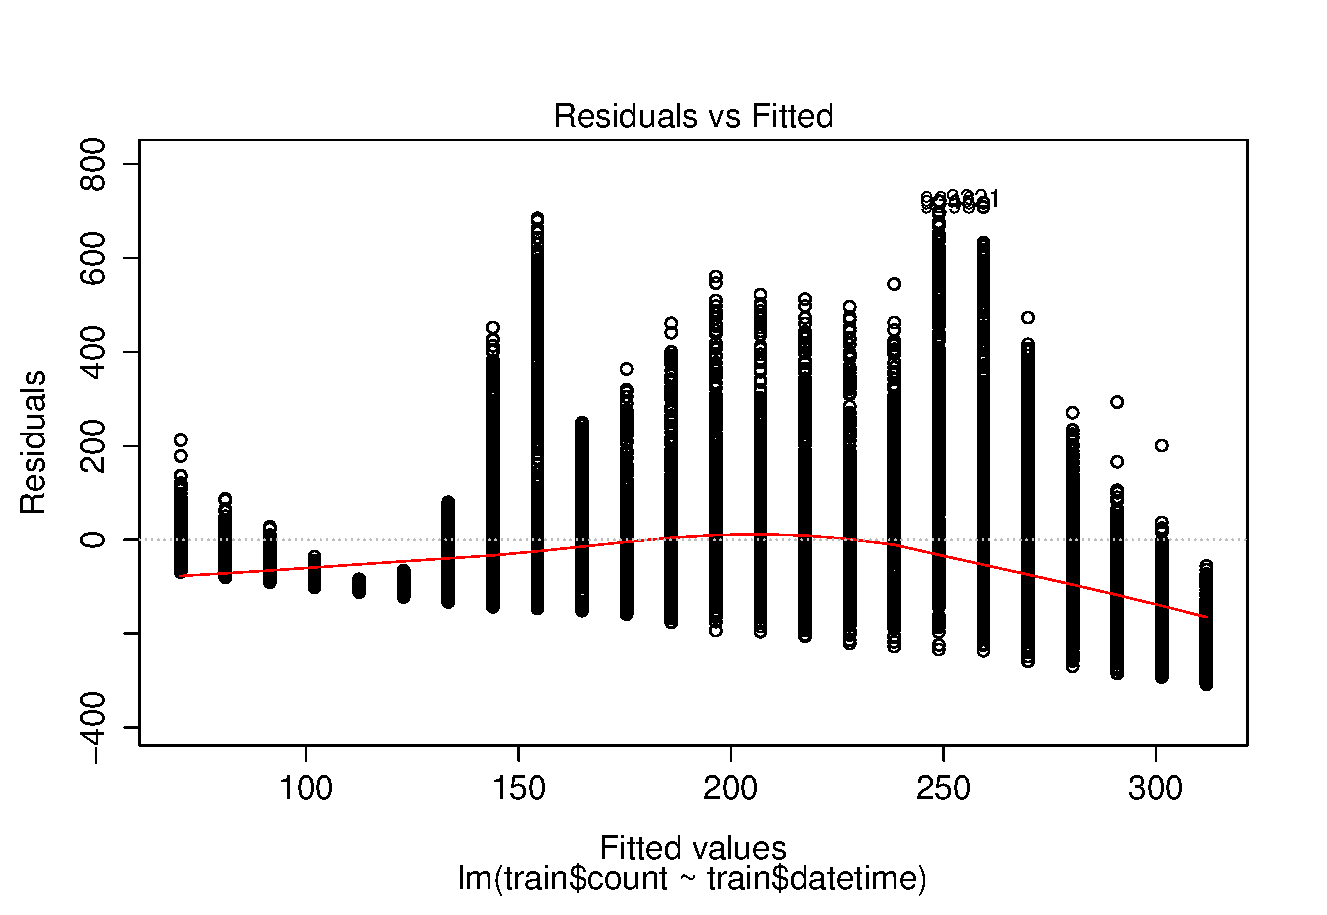
\includegraphics[width=.7\columnwidth]{images/simple-linear-model-plot.eps}
  \caption{Grafico dei residui per il modello lineare con
  \texttt{train\$datetime}}\label{fig:simpl-mod-lin-residuals}
\end{figure}

\begin{figure}[H]
  \centering
  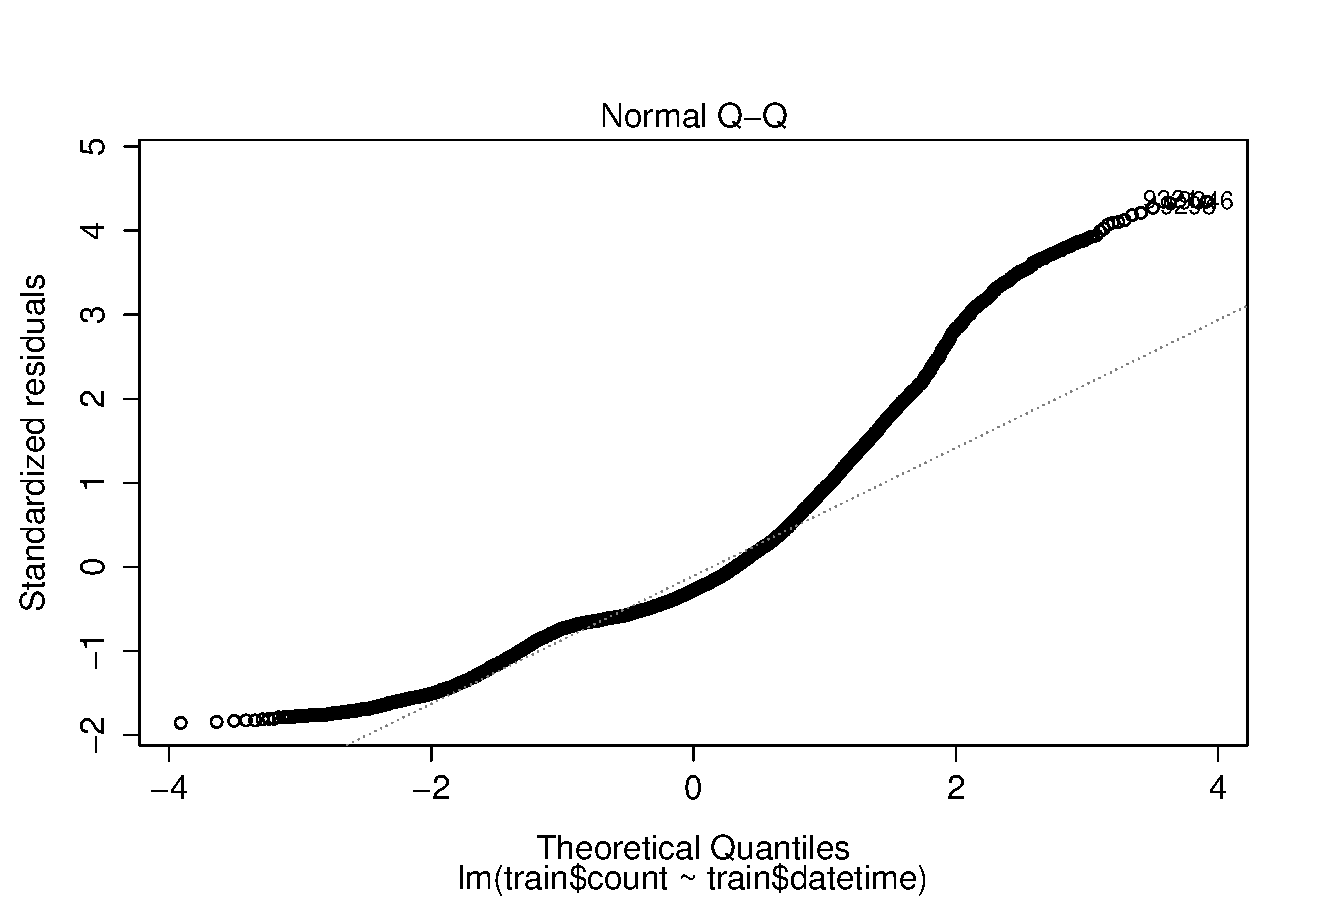
\includegraphics[width=.7\columnwidth]{images/simplest-linear-model-qqplot.eps}
  \caption{QQPlot per il modello lineare con
  \texttt{train\$datetime}}\label{fig:simpl-mod-lin-qqplot}
\end{figure}

\paragraph{Modelli con variabili esplicative trasformate} \mbox{}\\
Per rimediare a quanto detto sopra, si pensa a come introdurre nel modello
qualcosa che contribuisca a rendere la distribuzione degli errori più simile
a quella gaussiana.

Tale procedimento è totalmente giustificato dal fatto che si ritiene di poter
approssimare la variabilità di un comportamento umano come l'utilizzo del
\emph{Bike sharing} con una distribuzione normale.

Inizialmente il tentativo consiste nell'utilizzare un modello del tipo
$ y = \beta{}_0 + \beta{}_1 \cdot{} z + \epsilon{} $, dove z è la variabile
\texttt{train\$datetime} elevata al quadrato.

Questa strada però non porta i risultati desiderati: nella figura
\ref{fig:simpl-mod-lin-residuals} era ben visibile che i residui non erano
soddisfacenti poichè ``sbagliavano'' per eccesso. Infatti vi erano errori
significativi di sovrastima, mentre le sottostime erano numerose ma di valore
più contenuto.

Analizzando il modello ottenuto, si può infatti vedere che:

\begin{itemize}
\item l'errore standard dei residui è aumentato;
\item il grafico dei residui è molto simile a quello visto nel primo studio;
\item i quantili osservati per i residui si discostano ancora di molto da
  quelli di una distribuzione normale.
\end{itemize}

\paragraph{Modelli con variabili risposta trasformate} \mbox{}\\
Si procede dunque con un secondo tentativo, provando ad agire sul valore della
variabile risposta. Dagli stadi di analisi precedenti ormai è chiaro che
l'errore commesso era dovuto ad alcuni valori della variabile risposta che
erano piuttosto elevati.

Anzichè trasformare le variabili esplicative, quindi, forse è più conveniente
trasformare la variabile risposta in modo da attenuare i valori più alti di
questa:

\centering $ w = \beta{}_0 + \beta{}_1 \cdot{} x + \epsilon{} $
\flushleft dove $ w = log(y) $.

Questo modello risulta vincente, poichè l'errore standard dei residui passa da
166 a 1.333 e il grafico dei residui risulta più adeguato rispetto ad una
distribuzione normale, così come il QQPlot ora ha una distribuzione dei
quantili osservati molto più vicina a quella di una normale.

\begin{figure}[H]
  \centering
  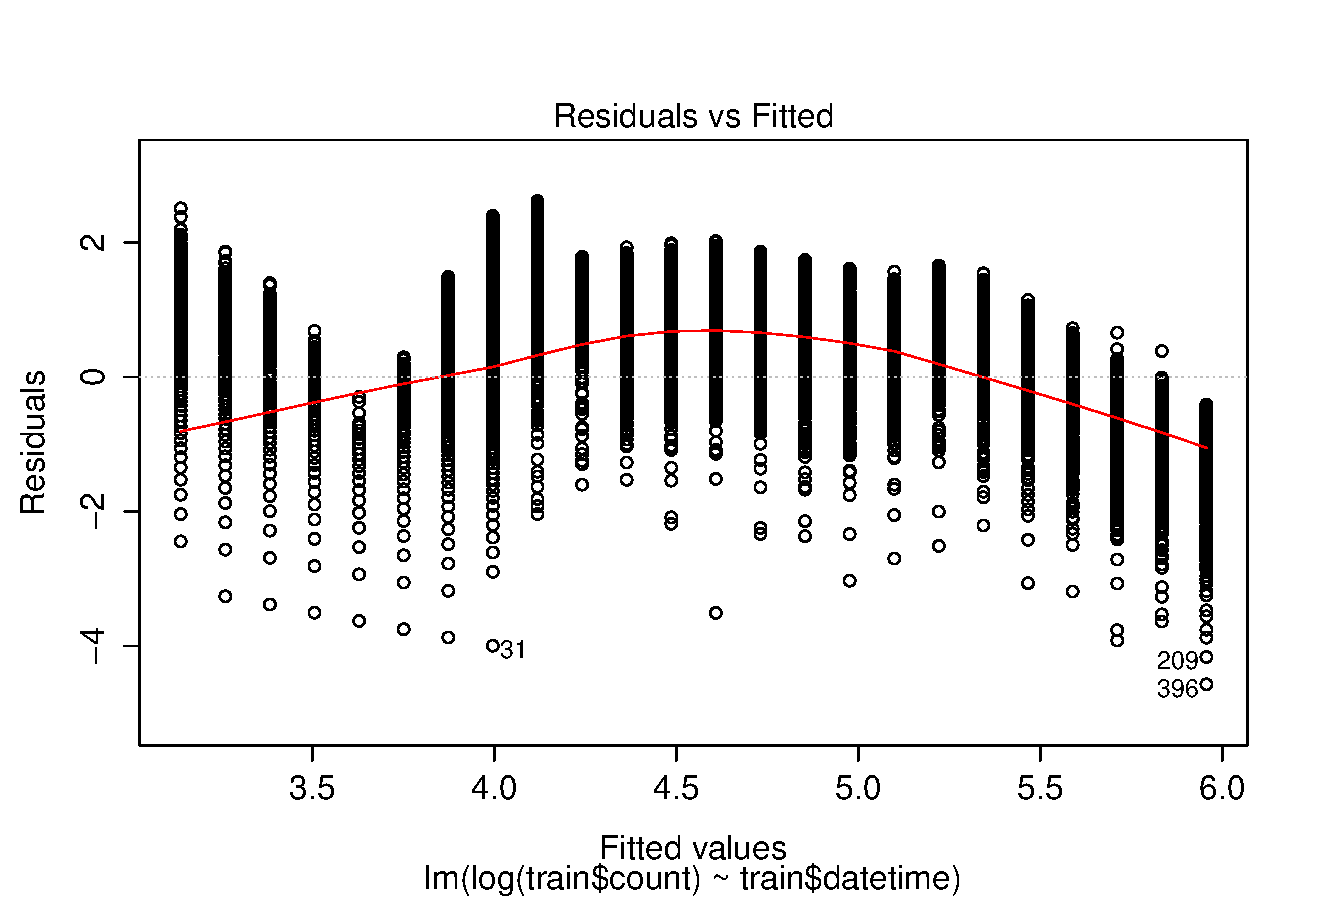
\includegraphics[width=.7\columnwidth]{images/simple-lm-log-residuals.eps}
  \caption{Grafico dei residui per il modello lineare migliorato con
  \texttt{train\$datetime}}\label{fig:simpl-lm-log-residuals}
\end{figure}

\begin{figure}[H]
  \centering
  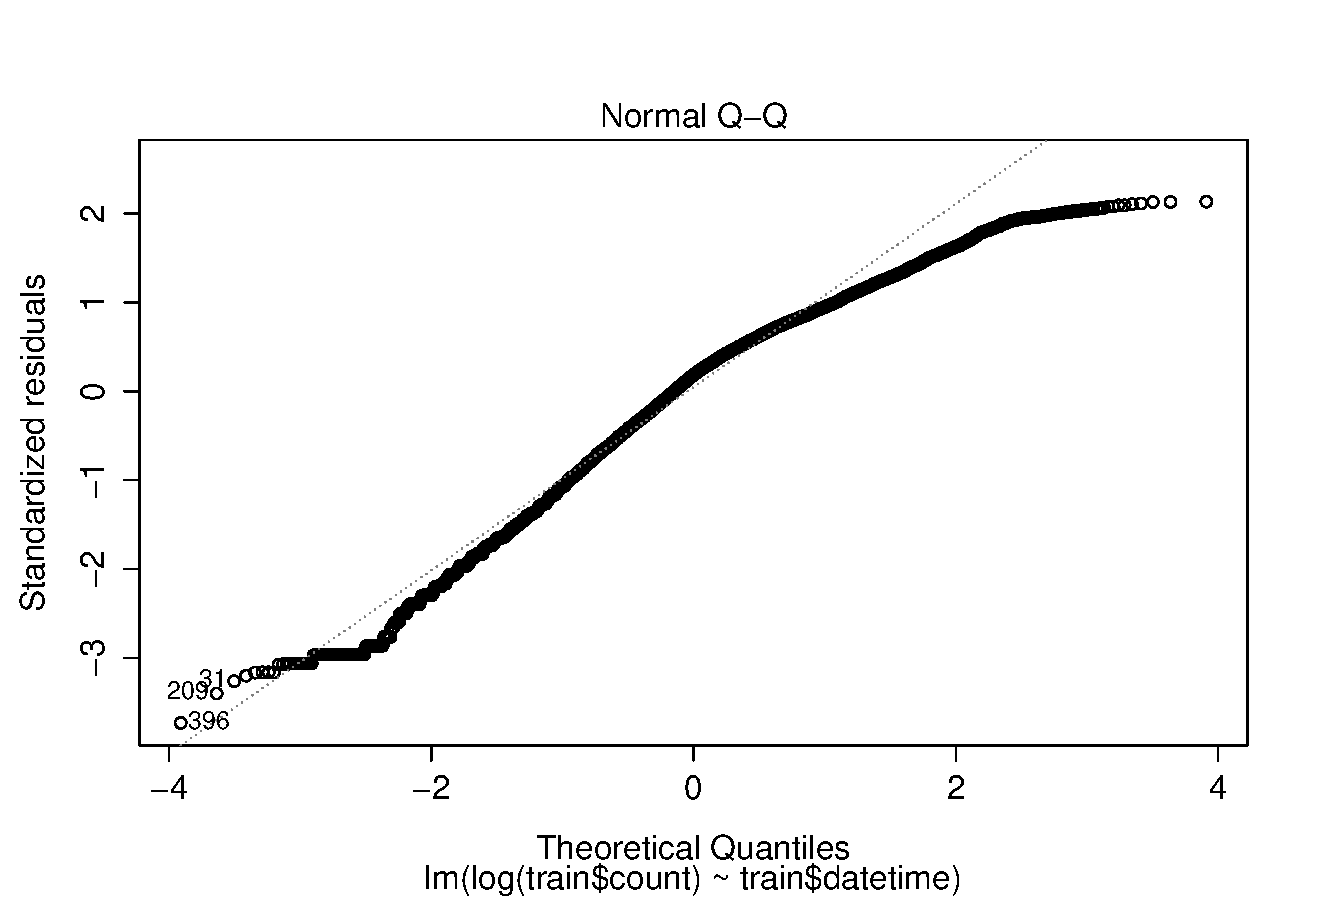
\includegraphics[width=.7\columnwidth]{images/simple-lm-log-qqplot.eps}
  \caption{QQPlot per il modello lineare migliorato con
  \texttt{train\$datetime}}\label{fig:simpl-lm-log-qqplot}
\end{figure}

\subsection{Modello lineare con \emph{forward stepwise selection}}\label{sec:mod-lin-fwd-sw}
Il modello di prima ha portato a discreti risultati, se non per il fatto che
utilizzava solamente una delle variabili esplicative.

Un approccio naïf potrebbe essere quello di inserire nel calcolo del modello
lineare tutte le variabili esplicative presenti nel set \texttt{train} e di
calcolare il modello lineare con il comando fornito da R.

Come è possibile vedere, ci sono alcune variabili che non sono significative e
altre che invece è sensato che appartengano al nostro modello:

\begin{figure}[H]
  \centering
  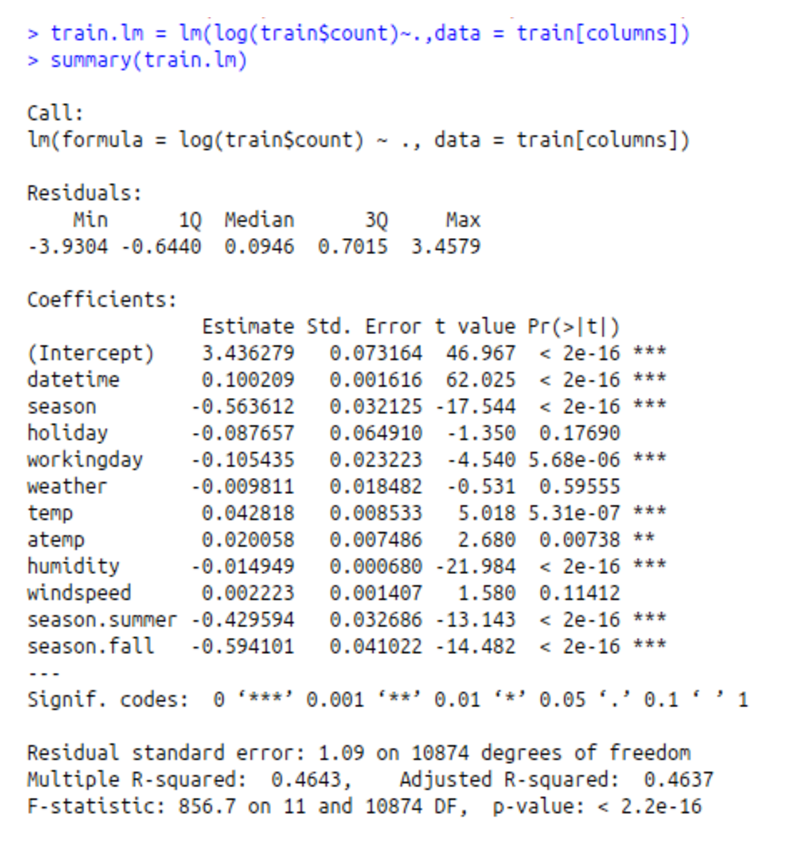
\includegraphics[width=.55\columnwidth]{images/lm-with-all-vars.eps}
  \caption{Modello lineare calcolato su tutte le variabili in modo
    non-ordinato}\label{fig:simpl-lm-log-qqplot}
\end{figure}

Tuttavia, anzichè provare manualmente qualsiasi combinazione di variabili
affinchè non si trovi il modello lineare migliore, si decide di automatizzare
il tutto con un paio di script:

\begin{itemize}
\item \texttt{linearModel.R} (sez. \ref{sec:script-linear-model}): questo
  script in pratica realizza quanto fatto nella prima parte dell'analisi
  tramite un modello lineare.
  \begin{enumerate}
  \item Dato il modello $ w = \beta{}_0 + \beta{}_1 \cdot{} x + \epsilon{} $,
  viene cercata la variabile esplicativa più significativa, confrontando la
  statistica F delle variabili \texttt{train\$[columns]} (ovvero le variabili
  esplicative);
  \item Nel frattempo, vengono stampate a video le variabili esplicative, il
  coefficiente di determinazione e la statistica F ottenuti usando questi come
  ``x'' per il modello;
  \item A questo punto, viene trovata la variabile più significativa, tale
  risultato viene stampato a video e questa viene usata per calcolare il
  miglior modello lineare con una variabile esplicativa;
  \item Il nome di questa variabile viene salvato in un array chiamato
  \texttt{already\_present} e viene invocato il secondo script.
  \item Alla fine dello script, il workspace viene pulito, lasciando solamente
  le variabili \texttt{train.lm} (il modello ricercato) e \texttt{train.lm2}
  (il modello con tutte le variabili esplicative oppure con una variabile non
  significativa presente oltre a quelle presenti in \texttt{train.lm}).
  \end{enumerate}
\item \texttt{linear\_model\_forward\_steps.R} (sez.
  \ref{sec:script-linear-model-fwd-steps}): questo script serve per iterare
  lungo le variabili esplicative al fine di inserire in modo incrementale le
  variabili più significative per il nostro modello.
  \begin{enumerate}
  \item All'inizio dello script, \texttt{train.lm} è il modello lineare con n
    variabili esplicative, dove n è il numero di volte che è stato invocato;
  \item Per ognuna delle variabili esplicative, viene eseguito un insieme di
    istruzioni. Se la variabile è già presente nel modello (e quindi in
    \texttt{already\_present}), viene saltata;
  \item Si procede calcolando il modello lineare aggiungendo alle variabili
    già presenti quella coinvolta nell'iterazione corrente;
  \item Viene eseguita l'ANalysis Of VAriance (\textbf{ANOVA}) sul nuovo
    modello;
  \item Tramite queste iterazioni, si trova la variabile più significativa da
    aggiungere al modello lineare presente all'inizio dello script;
  \item Tale variabile viene inserita solamente se contribuisce in modo
      significativo a migliorare il modello; per far questo, si confronta il
      suo p-value con una soglia stabilita a priori (nel nostro caso 5\%),
      impostata con lo script di popolamento (sez. \ref{sec:script-populate})
      nella costante \texttt{FWD\_SW\_THRESHOLD};
    \item Se la variabile è stata inserita, viene ricalcolato \texttt{train.lm}
      aggiungendo questa variabile, vengono stampate le variabili presenti nel
      modello e viene invocato ricorsivamente questo script;
    \item Quando non vi sono più variabili da aggiungere, il workspace viene
      pulito (facendo attenzione a non ripetere rimozioni su oggetti già
      cancellati) e in \texttt{train.lm} è presente il modello ricercato.
  \end{enumerate}
\end{itemize}

Di seguito vengono riportati i dati del modello lineare ottenuto tramite gli
script sopra descritti:

\begin{figure}[H]
  \centering
  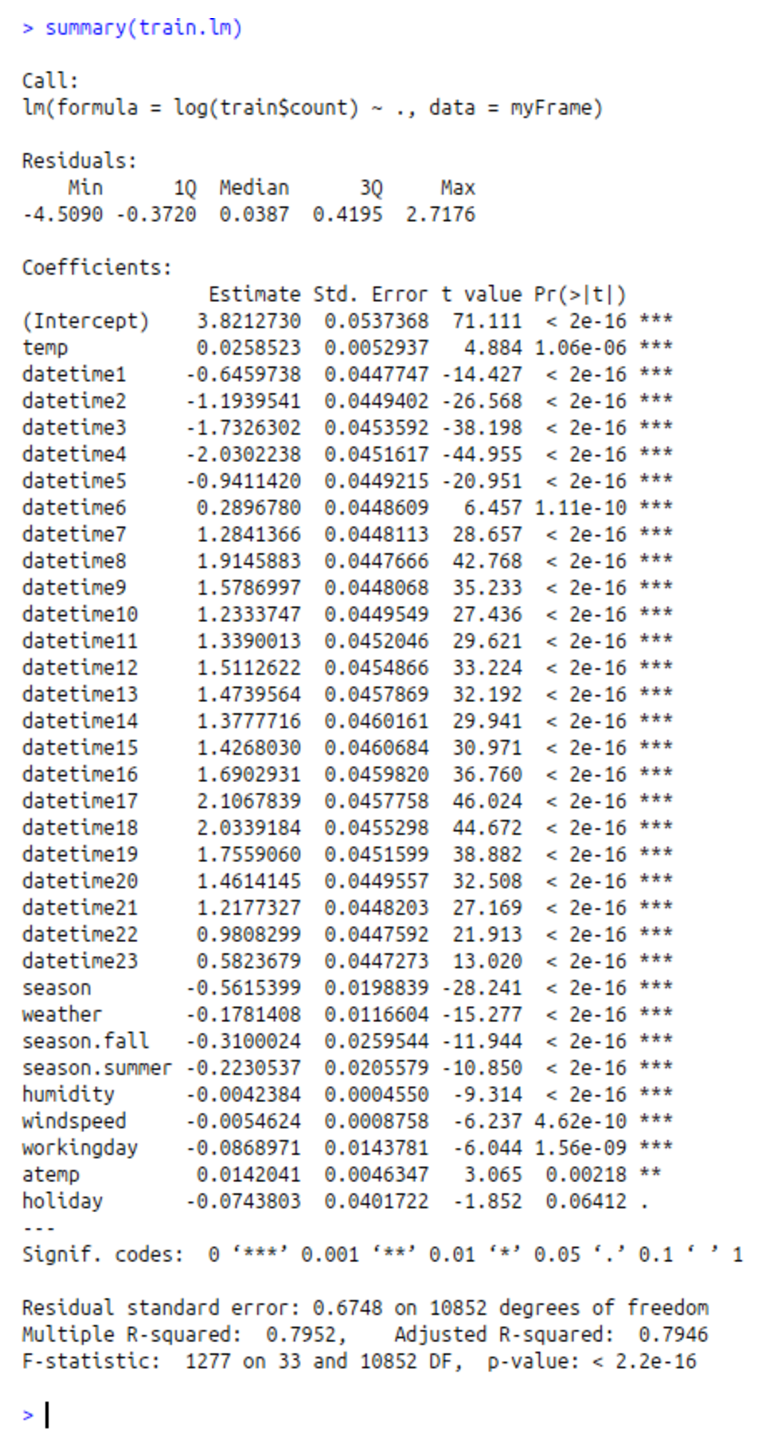
\includegraphics[width=.55\columnwidth]{images/lm-after-fwd-steps.eps}
  \caption{Modello lineare calcolato tramite forward-stepwise selection}
    \label{fig:lm-after-fwd-steps}
\end{figure}

\subsection{Stima ai minimi quadrati con filtro ricorsivo}
Anche se non richiesto dal problema, si è voluto rendere il calcolo del
modello lineare efficiente nel caso in cui il dataset non fosse composto da un
insieme di dati prefissati, ma da uno stream che continuasse a far pervenire
dati.

A tal riguardo è stato sviluppato uno script chiamato \texttt{KalmanFilter.R}
che lavora grazie a ortogonalizzazioni successive.

Tale algoritmo può essere paragonato ad un filtro di Kalman poichè anch'esso
cerca di valutare lo stato (più specificatamente, la relazione tra le
variabili esplicative e quella risposta) di un sistema dinamico (assumendo che
i dati arrivino tramite stream) le cui osservazioni si assume che siano
incorrelate, con distribuzione normale e a media nulla.

Oltre a ciò, ci si aspetta che la richiesta del servizio di \emph{Bike sharing}
segua un modello ``vero'', costante nel tempo e non casuale. In poche parole,
ci si aspetta che i vari valori $ \beta{}_i $ (dove $i$ è un indice relativo
alle variabili esplicative) abbiano stabilità asintotica.

Procediamo quindi con la descrizione per spiegare in cosa consiste tale filtro:

\begin{enumerate}
\item Prima di tutto vengono mescolati casualmente i dati presenti nella
  matrice di partenza, in modo tale da assicurare che il modello finale abbia
  valori vicini a quello trovato nella sezione \ref{sec:mod-lin-fwd-sw}
  indipendentemente dall'ordine in cui sono elaborate le righe della matrice
  \texttt{train};
\item Vengono generate una matrice X e si calcola il logaritmo della variabile
  risposta (per le analisi svolte nelle sezioni precedenti)
\item Inizialmente la matrice \texttt{V} che sarà utilizzata per le
  ortogonalizzazioni successive è la matrice identità, mentre $ \beta{} $, la
  colonna di coefficienti relativi alle variabili esplicative, viene calcolata
  utilizzando come variabile risposta il valore medio di \texttt{y};
\item Per tutte le righe in X, viene iterato un filtro ricorsivo su \texttt{V}
  con il quale si calcola la matrice H (\emph{Hat}) in base all'ultima
  osservazione arrivata per le variabili esplicative e, grazie a questa,
  aggiorna il vettore $ \beta{} $;
\item Al termine delle iterazioni, le righe di $ \beta{} $ vengono chiamate
  con gli stessi nomi delle variabili esplicative per favorirne il confronto
  con modelli ottenuti con strumenti automatici;
\item Vengono mostrati tre valori del vettore $ \beta{} $ e il modo in cui essi
  sono evoluti durante l'algoritmo ricorsivo: è possibile vedere che i
  coefficienti hanno stabilità asintotica.
\end{enumerate}

Di seguito vengono riportati i coefficienti di $ \beta{} $ che, se confrontati
con quelli in figura \ref{fig:lm-after-fwd-steps}, ci convincono che il filtro
ricorsivo abbia funzionato correttamente.

Oltre a questi coefficienti, vengono riportati i grafici in cui è possibile
vedere che i valori in $ \beta{} $ raggiungono i valori ``veri'' per numerosità
di osservazioni sufficientemente elevate.

\begin{figure}[H]
  \centering
  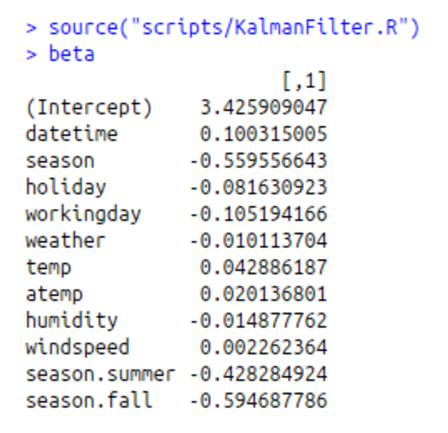
\includegraphics[width=.55\columnwidth]{images/kalman-beta.eps}
  \caption{Coefficienti calcolati tramite filtro ricorsivo}
    \label{fig:kalman-beta}
\end{figure}

\begin{figure}[H]
  \centering
  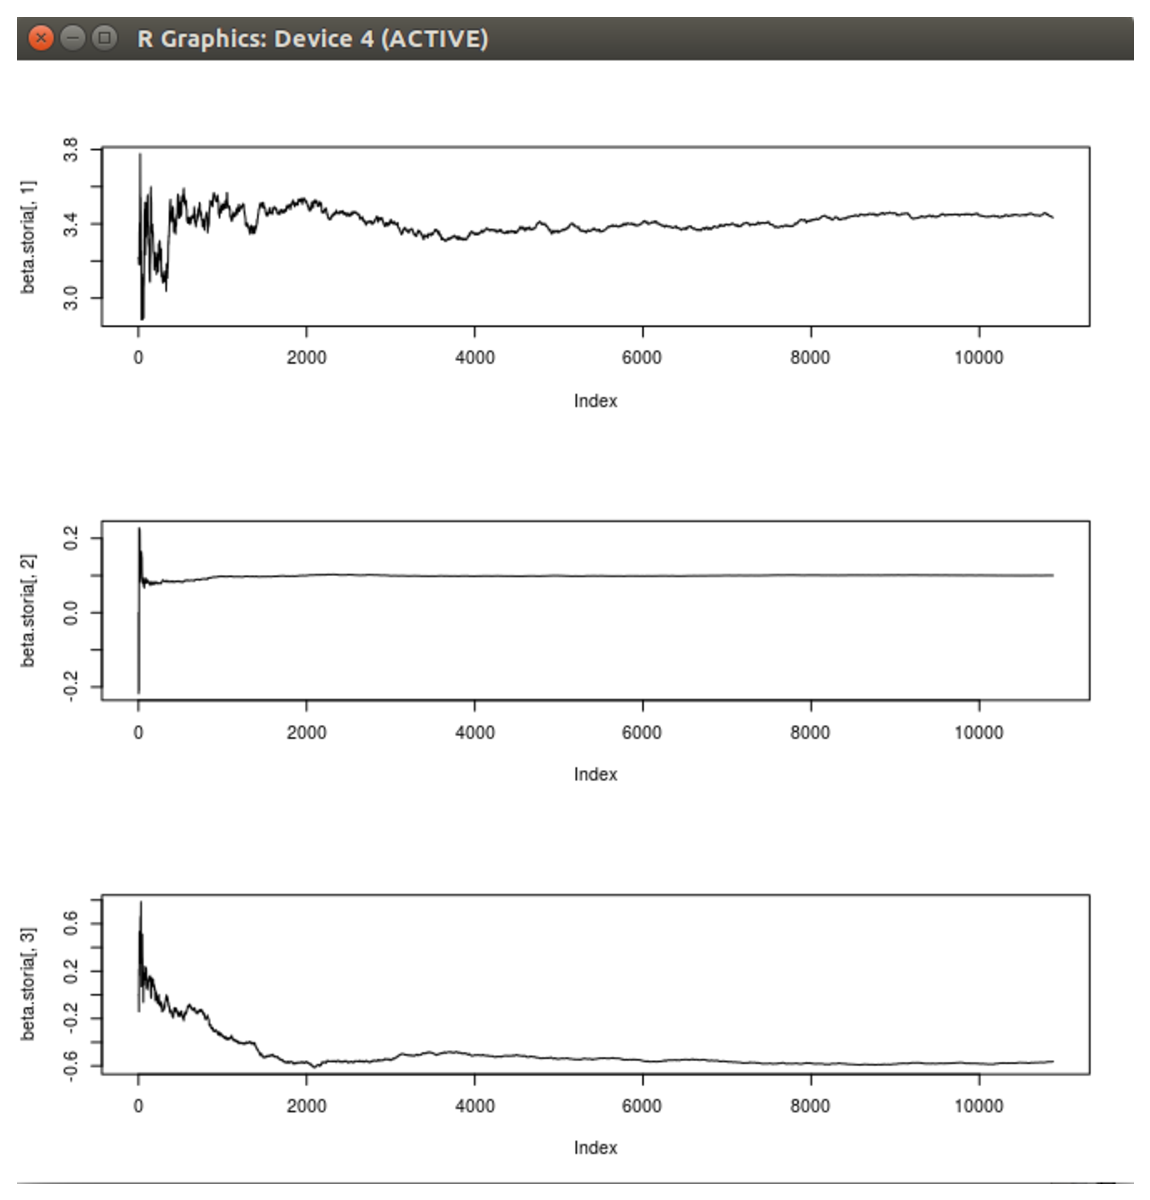
\includegraphics[width=.55\columnwidth]{images/kalman-asymptotic.eps}
  \caption{Stabilità asintotica del filtro ricorsivo}
    \label{fig:kalman-asymptotic}
\end{figure}

Si può notare come $ \beta{} $ contenga in realtà tutte le variabili e non solo
quelle più significative, stando a quanto trovato nella sezione
\ref{sec:mod-lin-fwd-sw}. Ciò è dovuto al fatto che non è strettamente
necessario seguire un ordine preciso per queste due fasi di analisi, tuttavia
come possibile sviluppo applicativo, se sorgesse la necessità, sarebbe
possibile combinare i due in modo tale che eseguendo \emph{forward-stepwise
selection} su una parte sufficientemente grande dei dati si riesca ad
individuare le variabili che sono significative e quelle che non lo sono, per
poi lasciare che il filtro ricorsivo gestisca lo stream di dati in input
calcolando il modello solamente per le variabili esplicative trovate nella
prima fase.
